\documentclass[british]{beamer}

\usepackage{default}
\usepackage[british]{babel}
\usepackage{epstopdf}
\usetheme{Madrid}
\usepackage{graphicx}
\usepackage{dirtytalk}
\usepackage{csquotes}
\usepackage{wrapfig}
\usepackage{tikz}
\usepackage{smartdiagram}

\begin{document}
%
\title[Document Semantic Similarity]
{Document Semantic Similarity}

\subtitle{TIS Project}

\author[A. Pirovano, F. Picciotti]
{Alberto Pirovano \and Francesco Picciotti}

\institute[PoliMi]
{
	Politecnico di Milano
}

\logo{
	
\includegraphics[height=1.7cm,trim={0 2cm 4.5cm 2cm},clip]
	{./Imgs/Politecnico-di-Milano-3-m8qw.eps}
	}	

\AtBeginSection[]
{
	\begin{frame}
		\frametitle{Outline}
		\tableofcontents[currentsection, currentsubsection]
	\end{frame}
}

\AtBeginSubsection[]{
	\begin{frame}
		\frametitle{Outline}
		\tableofcontents[currentsection, currentsubsection]
	\end{frame}
}

\maketitle

\section{State of art}

\begin{frame}{Introduzione}
	Le tecniche adottate attualmente per trovare la \textbf{similitudine semantica tra testi} si basano su tre approcci:
	\begin{enumerate}
		\item NLP Tradizionale
		\item Vector Space Model
		\item Deep Learning based 
	\end{enumerate}
\end{frame}
	
\subsection{NLP tradizionale}
	
\begin{frame}{NLP Tradizionale}
	Questo approccio si basa sull'utilizzo delle tradizionali tecniche di \textbf{Natural Language Processing} e si costituisce dei seguenti step:
	\begin{itemize}
		\item Cleaning dei dati
		\item Pos-Tagging
		\item Stemming o Lemmatisation
		\item Parsing
		\item Ontologia
	\end{itemize}
	Tuttavia, dato che il nostro lavoro \`{e} molto \textbf{sensibile} e \textbf{dipendente} dalla qualit\`{a} dei tool utilizzati, abbiamo trovato alcune consistenti \textbf{criticit\`{a}} riguardanti:
	\begin{itemize}
		\item \textbf{L'affidabilit\`{a}} del Pos-Tagger italiano di TreeTagger
		\item \textbf{Reperire} una Ontologia e un parsing toll per la  lingua italiana
	\end{itemize}
\end{frame}

\begin{frame}{NLP Tradizionale}
	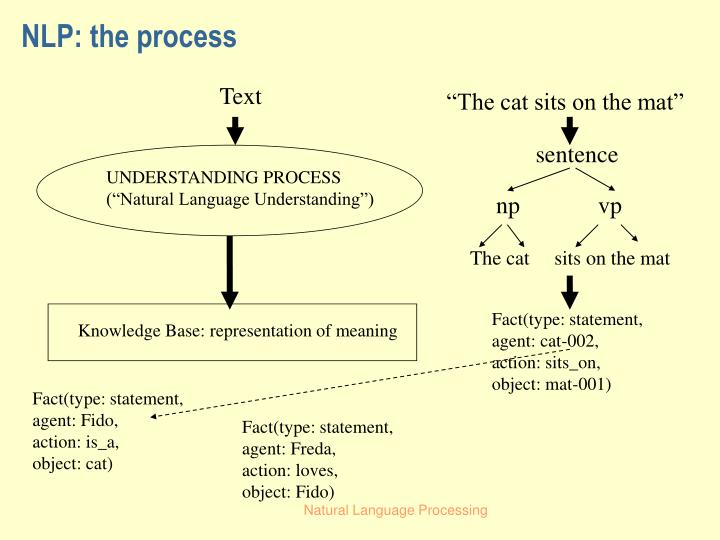
\includegraphics[width=0.9\textwidth, height=0.85\textheight]{./Imgs/nlp-the-process.jpg}
\end{frame}
	
\subsection{Vector Space Model}
	
\begin{frame}{Vector Space Model - Explanation}
	\begin{wrapfigure}{r}{0.4\textwidth}
		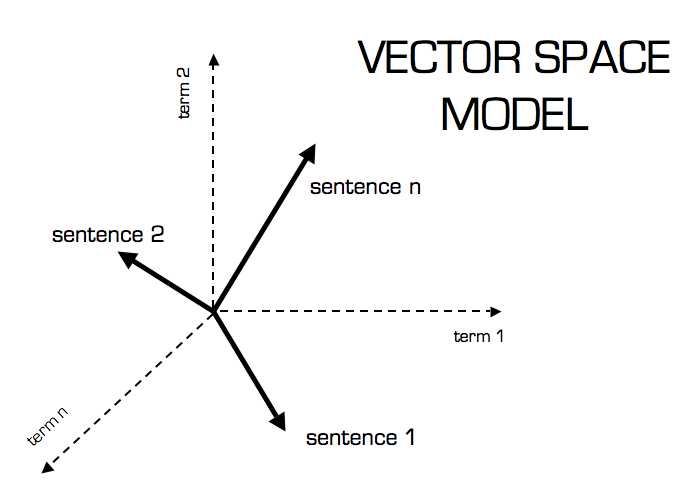
\includegraphics[width=1.1\linewidth,height=0.4\textwidth]{./Imgs/vector_space.png}
	\end{wrapfigure}	
	Differentemente dal precedente, questo approccio ha le sue basi nello sviluppo di una \textbf{rappresentazione geometrica e vettoriale} per i documenti testuali.
	\textbf{Documenti e query} sono rappresentati da vettori con un numero di elementi pari al numero di termini presenti nel vocabolario.
	Tipicamente i termini sono le parole distinte presenti nell'insieme di documenti, tuttavia un termine pu\`{o} essere anche una \textbf{keyword} o una \textbf{frase}.
	A valle di questa rappresentazione vengono spesso utilizzate le \textbf{operazioni vettoriali} per confrontare due \textbf{documenti}.
\end{frame}

\begin{frame}{Vector Space Model - Encoding}
	Nel vector space model proposto da \textbf{Salton, Wong and Yang} i vettori sono composti da \textbf{weights}, ognuna associata ad un termine del dizionario e calcolata tramite \textbf{tf-idf}.\par
	Considerando un \textbf{documento \(d_j\)}, questo viene rappresentato tramite un \textbf{vettore \(d_j\)}: \par
	\begin{itemize}
		\item \(d_j = (w_{1,j}, w_{2,j}, ..., w_{t,j})\) \textbf{dove}:
		\(w_{i,j} = tf_{t,d} * \log_{}{\frac{|D|}{|\left \{d' \in D | t \in d'\right \}|}}\)
	\end{itemize}
	
\end{frame}

\begin{frame}{Vector Space Model - LSA}
	
	\textbf{Latent Semantic Analysis} \`{e} una tecnica di \textbf{Topic Modelling} che si colloca a valle del \textbf{document encoding} con \textbf{tfidf}. 
	
	\`{E} una tecnica di \textbf{feature extraction} (PCA) che permette di migliorare significativamente la qualit\`{a} di un lavoro di \textbf{clustering}, dato che la metrica non considera la differenza tra \textbf{features non importanti}.
	
	Questa procedura viene usata per astrarre una categorizzazione di un \alert{set di documenti} in un \alert{set di topic} o anche per osservare le parole che descrivono un certo topic.
	
	Si basa sulla creazione di una \textbf{Document-Term Matrix} nella quale le \textbf{righe} rappresentano le parole del \textbf{Bag Of Words} e ha una \textbf{colonna} per \textbf{documento} nel corpora.
	
	Il cuore di questa procedura sta nella \textbf{riduzione della dimensionalit\`{a}} di questa matrice tramite \textbf{SVD}.
	
\end{frame}

\begin{frame}{Vector Space Model - LSA - SVD}
	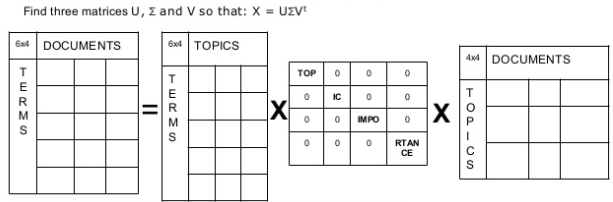
\includegraphics[width=0.9\textwidth, height=0.4\textheight]{./Imgs/LSA1}
\end{frame}

\begin{frame}{Vector Space Model - LSA}
	Questa procedura ci permette di:
	\begin{itemize}
		\item \textbf{Estrarre} quanti topic desideriamo da un set di documenti.
		\item \textbf{Conoscere} la rilevanza di un certo topic dopo averlo estratto, in questo modo siamo in grado di fermare il processo di estrazione quando i topic cominciano a diventare poco significativi.
		\item \textbf{Categorizzare} documenti in topic
		\item \textbf{Descrivere} topics con le parole del \textbf{Bag Of Words}.
	\end{itemize}
\end{frame}

\begin{frame}{Vector Space Model - LSA - Example}
	In questo esempio possiamo osservare la riduzione di dimensionalit\`{a}.
	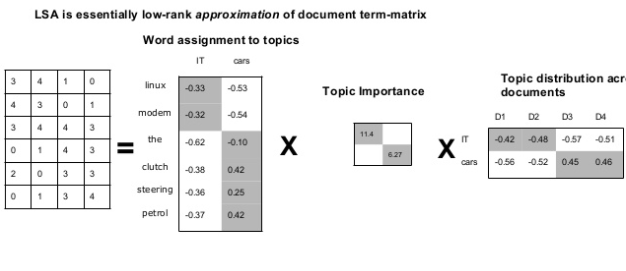
\includegraphics[width=0.9\textwidth, height=0.5
	\textheight]{./Imgs/LSA2}\\
	Il processo di LSA permette di costruire le 3 matrici che vediamo sopra, ognuna con una sua utilit\`{a}:
	\begin{enumerate}
		\item \textbf{Word assignment to topics}
		\item \textbf{Topic importance}
		\item \textbf{Topic distribution across documents}, \`{e} la nuova \textbf{Document-Term Matrix}.
	\end{enumerate}
\end{frame}

\begin{frame}{Vector Space Model - Algorithm}
	Riassumendo, possiamo individuare i seguenti \textbf{passaggi}:
	\begin{enumerate}
		\item Cleaning dei dati (Stemming o Lemmatisation)
		\item Vectorization using TF/IDF
		\item LSA (optional)
		\item Clustering using similarity measure (Cosine, Pearson, ...)
	\end{enumerate}
\end{frame}

\begin{frame}{Vector Space Model - LSA - Performance}
	Come possiamo vedere nella figura, utilizzare le classiche tecniche di \textbf{clustering} senza \textbf{LSA} pu\`{o} portare una riduzione rilevante delle \textbf{performances}:
	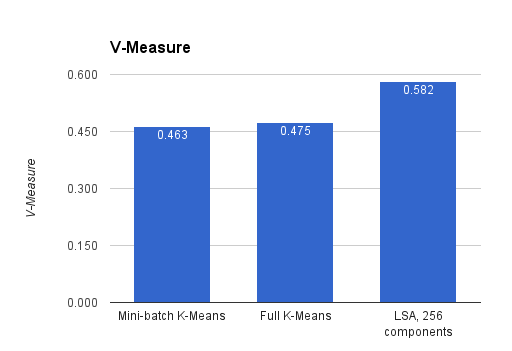
\includegraphics[width=0.9\textwidth, height=0.7\textheight]{./Imgs/LSAperf}
\end{frame}

\begin{frame}{Vector Space Model (con LSA) - Pros and Cons}	
	\begin{columns}
		\column{0.4\textwidth}
		\\
		\underline{Pros:}
		\begin{itemize}
			\item Modello semplice basato sull'\textbf{algebra}.
			\item Le \textbf{weights} non sono binarie.
			\item Permette di calcolare un grado di \textbf{similarit\`{a} continuo}.
		\end{itemize}
		\column{0.6\textwidth}
		\underline{Cons:}
		\begin{itemize}
			\item Non adatto a trattare \textbf{lunghi documenti}, infatti a causa della alta \textbf{dimensionalit\`{a}} il valore \textbf{tfidf} dei compoenti si riduce, riducendo il \textbf{dot-product}.(LSA fixes)
			\item \textbf{Fortemente sensibile a Falsi Negativi}, infatti documenti nello stesso \textbf{contesto} ma con diversa terminologia non saranno considerati simili.(LSA partially fixes)
			\item Perdiamo \textbf{l'ordine delle parole}.
			\item \textbf{Pre-processing} dipendente.
		\end{itemize}
	\end{columns}
\end{frame}
\iffalse
\begin{frame}{...limiti?}
	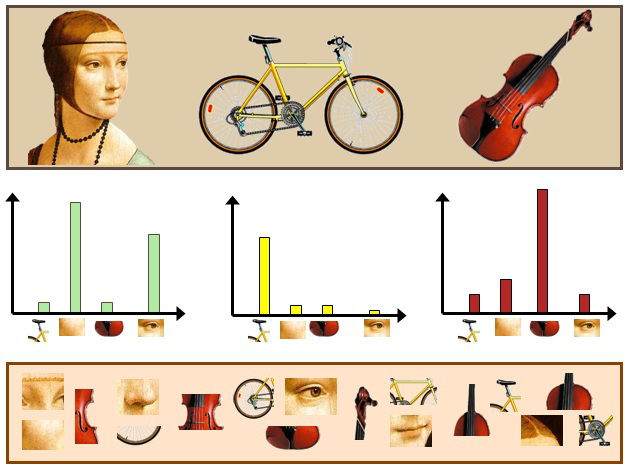
\includegraphics[width=0.9\textwidth, height=0.8\textheight]{./Imgs/bow-example.jpeg}
\end{frame}
\fi
\subsection{Deep Learning}

\begin{frame}{Deep learning based}
	
	Il terzo approccio che proponiamo \`{e} molto diverso dai precedenti, infatti si basa sull'utilizzo di \textbf{neural networks}.
	La fondamentale differenza \`{e} che, mentre il secondo \textbf{definiva un algoritmo} per determinare le rappresentazioni vettoriali delle parole (tfidf), questo \textbf{definisce una neural network} che con la task di imparare quell'algoritmo dai dati.
	Questa \textbf{NN} pu\`{o} essere \textbf{costruita} in due diversi modi, ognuno dei quali descrive \textbf{come} imparare la \textbf{word-representation} per ogni parola:
	\begin{itemize}
		\item \textbf{Continous Bag Of Words model}
		\item \textbf{Skip Grammar model}
	\end{itemize}
	Dato che il processo di apprendimento \`{e} \textbf{unsupervised}, questi modelli permettono di \textbf{determinare la task} tramite la definizione di un target per ogni input.
\end{frame}
	
\begin{frame}{Deep Learning based}
	Questa tecnica quindi si basa su 3 ambiti:
	\begin{figure}[!hf]
		\centering
		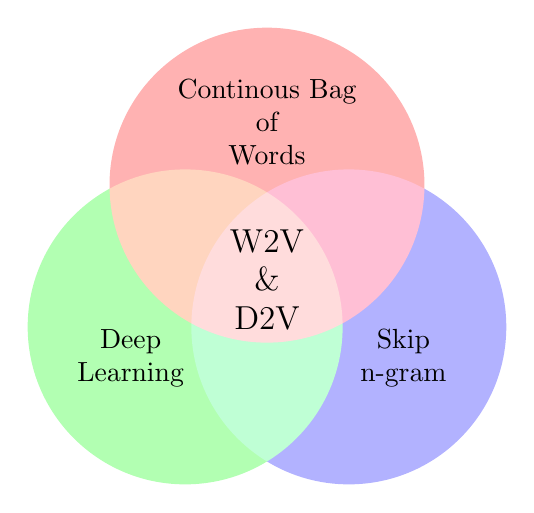
\begin{tikzpicture}
		\begin{scope}[blend group = soft light]
		\fill[red!30!white]   ( 90:1.2) circle (2);
		\fill[green!30!white] (210:1.2) circle (2);
		\fill[blue!30!white]  (330:1.2) circle (2);
		\end{scope}
		\node at ( 90:2)    
		[font= \normalsize, align= center]
		{Continous Bag \\ of \\ Words};
		\node at ( 210:2)   
		[font= \normalsize, align= center]
		{Deep \\ Learning};
		\node at ( 330:2)   
		[font= \normalsize, align= center]
		{Skip \\ n-gram};
		\node [font=\large, , align= center] {W2V \\\& \\D2V};
		\end{tikzpicture}
	\end{figure}
\end{frame}
	
\begin{frame}{Deep Learning based: Word2Vec \& Doc2Vec}
	Questo metodo \`{e} stato implementato da \textbf{Google} sotto il nome di \textbf{Word2Vec} e \textbf{Doc2Vec}.
	Il primo permette di determinare le \textbf{relazioni semantiche} che un particolare \textbf{corpus di testi} assegna ad un \textbf{Bag Of Words} di parole.
	\textbf{Doc2Vec} invece \`{e} una tecnica che si configura come una \textbf{estensione di Word2Vec} la quale, preso in ingresso un set di documenti (corpora), genera un \textbf{grado di similarit\`{a}} reciproco.
\end{frame}

\begin{frame}{Deep Learning based - Pros and Cons}
	Dopo una ampia \textbf{discussione}, seguita da una approfondita \textbf{analisi critica} di questi due approcci, siamo giunti alle seguenti \textbf{conclusioni}, che in termini di pro e contro si possono riassumere nel seguente modo:
	\begin{columns}
		\column{0.5\textwidth}
		\\
		\underline{Pros:}
		\begin{itemize}
			\item Molto meno dipente da un preprocessing
			\item \textbf{Context-aware}
			\item Combina il metodo \textit{Geometrico} con quello \textit{NLP Tradizionale}
			\item \textbf{Non sfrutta una ontologia, ma la \alert{crea}} 
			\item \textbf{\alert{Language independent}}
		\end{itemize}
		\column{0.5\textwidth}
		\underline{Cons:}
		\begin{itemize}
			\item Tecnica \textbf{unsupervised}
			\item Necessit\`{a} di un esperto per \textbf{validare} la similarit\`{a}
			\item Pu\`{o} risultare in \textbf{GIGO} system (Garbage In Garbage Out)
		\end{itemize}
	\end{columns}
\end{frame}
	
\section{Data Preparation}

\begin{frame}{Dataset}
	\begin{displayquote}
		"Preprocessing is 80\% of NLP work"
		 
		\begin{flushright}
			\textit{Lev Konstantinovskiy}
		\end{flushright}
	\end{displayquote}
	Il \textbf{dataset} si suddivide in due corpora: 
	\begin{itemize}
		\item il corpus del \textbf{Sole 24 Ore} con 3265 articoli, di cui 31 non hanno body
		\item il corpus di \textbf{Radiocor} con 6916 articoli
	\end{itemize}
	Il corpus prima del \textbf{preprocessing} contiene quindi 10150 articoli. \par
	Togliendo i \textbf{duplicati} otteniamo 9283 articoli, cio\'{e} ci sono 867 articoli duplicati.
\end{frame}

\subsection{Preprocessing}

\begin{frame}{Pipeline completa}
	\begin{center}
		\smartdiagramset{
			module minimum width= 5cm, 
			text width= 4.5cm,
			font= \tiny,
			set color list={blue!50!cyan,green!60!lime,orange!50!red,red!80!black},
			back arrow disabled=true}
		\smartdiagram[flow diagram: horizontal]{Cleaning del testo,Tokenizzazione e rimozione punteggiatura, Rimozione stopwords e POS-tagging del testo,Lemmatizzatione,Merge di verbi passivi composti}
	\end{center}
\end{frame}

\subsection{Cleaning del testo}

\begin{frame}{Cleaning pipeline}
	\begin{center}
			\smartdiagramset{
				module minimum width= 5cm,
				module minimum height= 0.1cm, 
				text width= 5cm,
				module y sep= 0.8cm,
				font= \tiny,
				set color list={blue!50!cyan,green!60!lime,orange!50!red,red!80!black},
				back arrow disabled=true}		
			\smartdiagram[flow diagram: vertical]{Lowercase di ogni lettera, Escape di caratteri unicode non stampabili, Tokenizzazione numeri percentuali, Rimozione preposizioni contratte, Tokenizzazione parola s24, Unificazione di espressioni di quantit\`{a}, Rimozione di intestazione di articolo, Rimozione di interruzione pagina, Rimozione chiusura aricolo, Rimozione urls e tags html}
	\end{center}
\end{frame}

\section{Word2Vec}

\begin{frame}{Hello}
	Qui speghiamo per bene come funziona word2vec
\end{frame}

\section{Doc2Vec}

\begin{frame}{Hello}
	Qui speghiamo per bene come funziona doc2vec
\end{frame}
\end{document}
